\pagestyle{empty}
\cleardoublepage
\pagestyle{fancy}
\chapter{Decomposição de domínios}\label{cap2}

Em Computação de Alto Desempenho, é conhecido que, para um bom algoritmo paralelo executar, é preciso uma boa estratégia para a divisão da entrada e para a junção das várias soluções ao final. 

Há ainda a preocupação com a distribuição das tarefas entre os processadores, levando em conta que, ao final todos eles devam ter realizado uma quantidade similar de processamento. Isso significa que a carga foi devidamente balanceada entre os processadores.

Nesse capítulo, irei mostrar o que se tem feito nos últimos anos nessa área de subdivisão de domínios, focando nas vantagens e desvantagens de cada técnica apresentada.


%\section{Introdução}\label{cap2:intro}
\section{Decomposição baseada no centro de densidade}

Em \cite{bib:Pirzadeh09}, é descrita uma técnica baseada em Avanço de Fronteiras e Avanço de Camadas. Essa é uma técnica tridimensional mas pode ser adaptada para uma versão bidimensional.

Primeiramente, é gerada a malha de superfície nos pontos dados como entrada. Logo em seguida, é feita uma estimativa de carga nos subdomínios utilizando uma \textit{octree}. Se necessário, serão criados planos de partições que dividem o domínio em regiões com cargas aproximadamente iguais. 

As posições destes planos são definidas através do centro de densidade da malha. Esse centro indica onde a massa efetiva do sistema está concentrada.

Em seguida, são identificadas as faces que interceptam o plano de partição e uma malha parcial é gerada na região do plano de corte. Depois disso, para cada lado da partição, são agrupadas as faces dos novos subdomínios. Esse processo é repetido até que um número máximo de subdivisões tenha ocorrido. Ao final da execução, tem que ser realizada uma junção de todas as submalhas. A Figura~\ref{fig:imagem1} ilustra os principais passos dessa técnica.

 \begin{figure}[htbp]
     \centering
     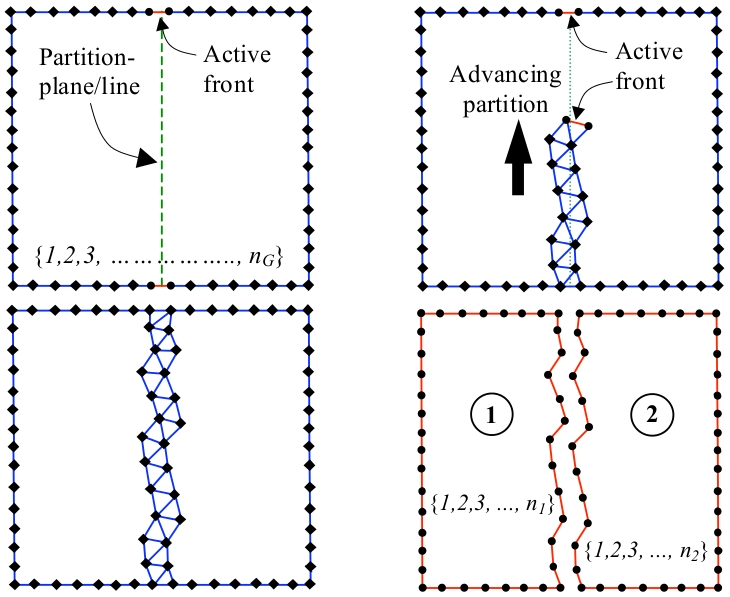
\includegraphics[width=0.8\textwidth]{imagem1}
     \caption{Os principais passos da técnica de \cite{bib:Pirzadeh09}.}
     \label{fig:imagem1}
 \end{figure}
 
 Como vantagens dessa técnica podemos citar que a utilização de avanço de camadas entre as partições faz com que a malha gerada seja praticamente idêntica a uma malha gerada sequencialmente, ou seja, não são gerados padrões entre as partições do domínio. Outra vantagem é que não é necessário nenhum pré-processamento para definir ou construir as partições.

\section{Decomposição baseada na distância/volume/centro de massa}
 
Em \cite{bib:Ivanov06}, foi desenvolvido um algoritmo baseado em Delaunay em que o posicionamento do plano de corte é definido pelo centro de massa e pela matriz de inércia. O plano de corte é um plano perpendicular a um eixo que segue uma das três definições:

\begin{itemize}
  \item Planos criados são equidistantes;

  \item Volume entre os planos são iguais;

  \item Passa pelo centro de massa.
\end{itemize}

A escolha do critério utilizado para criar os subdomínios vai depender da geometria da entrada. Dependendo da entrada, um critério pode ser melhor que outro, isso depende do conhecimento do usuário. Na Figura~\ref{fig:imagem2}, as três formas de decomposição são apresentadas.

Após ter o plano de corte definido, é feita uma suavização da seção de corte e a sua triangulação para, posteriormente, serem geradas as malhas nos subdomínios. Um problema bem visível nesse método é que para se ter um bom plano de corte é preciso ter um modelo com uma geometria bem comportada, sem forma côncava, alongada ou afinada.

 \begin{figure}[htbp]
     \centering
     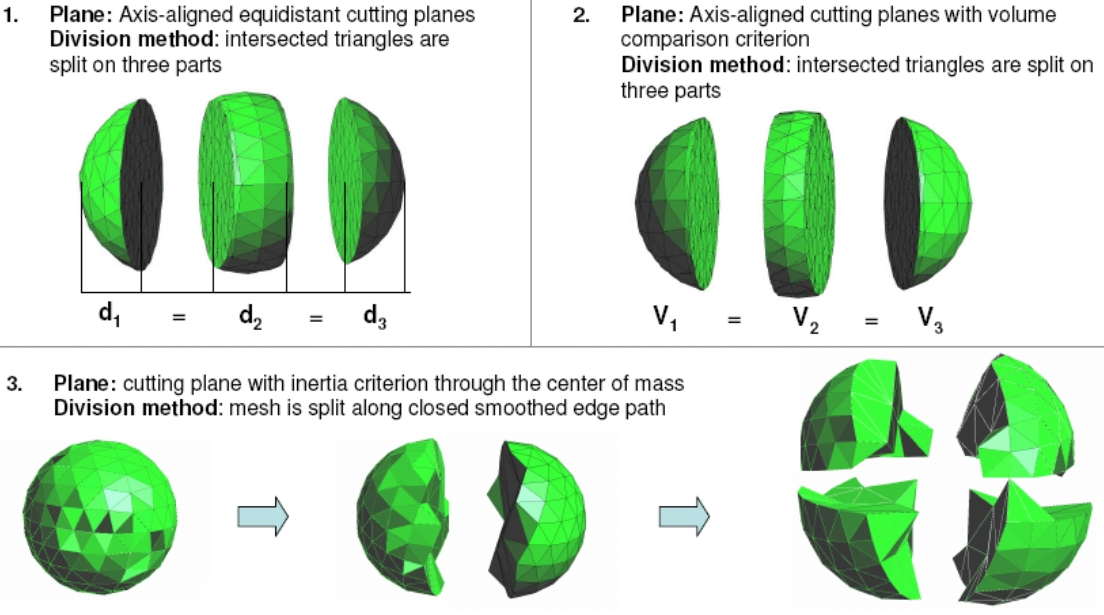
\includegraphics[width=0.9\textwidth]{imagem2}
     \caption{As 3 formas de particionar. 1 - planos equidistantes. 2 - volume dos subdomínios iguais. 3 - centro de massa \cite{bib:Ivanov06}.}
     \label{fig:imagem2}
 \end{figure}

Uma solução parecida é a apresentada em \cite{bib:Lammer00}, em que o plano de corte é traçado da mesma maneira, porém em duas dimensões, ou seja, um eixo de corte. Este eixo é usado para dividir o domínio recursivamente. A partir do eixo, uma aresta é formada, e os valores nos seus pontos extremos são interpolados dos valores dados como entrada. Quando o número de subdomínios for igual ao número de processadores, uma malha de Delaunay é gerada em cada interior.

\section{Decomposição baseada em \textit{octree}/\textit{quadtree}}

Em \cite{bib:deCougny99}, a entrada do algoritmo é o contorno de um objeto. Cada processador terá parte de uma \textit{octree} distribuída, que define planos de corte do domínio. A malha das células internas é gerada concorrentemente com \textit{templates}. A região entre o contorno e as células internas é preenchida por uma técnica de avanço de fronteira, onde são gerados os elementos internos a uma região delimitada pelos planos de corte. Por último é feita a conexão das malhas dos dois lados de cada plano e de suas intersecções.

Na técnica de \cite{bib:Lohner01}, é gerada uma \textit{octree} grosseira com relação ao contorno dado como entrada. Então, as células que contêm a parte da fronteira que gerará os menores elementos são identificadas. Assim, partes da malha, correspondentes a cada célula, são geradas simultaneamente por avanço de fronteira, de maneira que cada parte da malha gerada não possa cruzar as extremidades da célula que a contém. Então, cada octante sofre um pequeno deslocamento na diagonal com o intuito de gerar mais elementos. Esse deslocamento elimina quase todas as faces entre duas ou mais células e diminui o tamanho da fronteira para o próximo passo. Assim, a nova fronteira é encontrada, uma nova \textit{octree} é construída para ela, e o procedimento é repetido, até que não seja mais possível gerar malha.

Em \cite{bib:Larwood03}, é apresentada uma técnica de decomposição de domínio que tem como entrada uma triangulação de borda. Para saber quais subdomínios devem ser divididos, o autor usa um critério baseado na quantidade de faces por subdomínio. A decomposição é feita recursivamente usando uma \textit{octree} caso seja tridimensional ou uma \textit{quadtree} caso seja bidimensional, verificando sempre se o número de faces de um subdomínio é menor do que o limite estipulado, e, enquanto a verificação for falsa, a decomposição ocorre. A quantidade máxima de subdivisões está limitada por uma constante maior que o número de processadores disponíveis. Isso evita a criação excessiva de partições e permite que um processador possa receber mais de uma tarefa ao longo da execução.

Para evitar a criação de elementos ruins, é feita uma verificação no corte baseada no ângulo do vetor normal do plano de corte com a normal dos triângulos, de forma que o plano de corte não possa passar por triângulos com ângulo menor do que uma tolerância. Caso essa verificação falhe, a \textit{octree} (\textit{quadtree}, em 2D) sofre um deslocamento em um dos eixos. A Figura~\ref{fig:imagem3} mostra um exemplo onde alguns planos de corte falham nos testes.

 \begin{figure}[htbp]
     \centering
     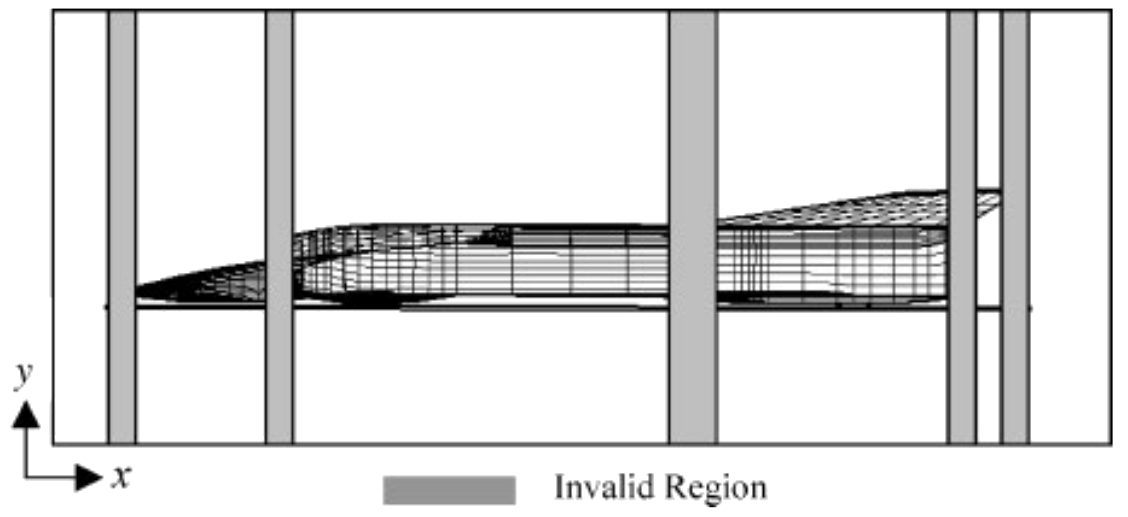
\includegraphics[width=0.9\textwidth]{imagem3}
     \caption{Regiões de corte inválidas em cinza \cite{bib:Larwood03}.}
     \label{fig:imagem3}
 \end{figure}

\section{Decomposição baseada no eixo mediano}

O eixo mediano é uma maneira de descrever a forma de um objeto, e é utilizado para garantir uma decomposição de domínio com separadores que formam bons ângulos com as bordas.

Em \cite{bib:Leonidas06}, é apresentada uma técnica bidimensional que utiliza a triangulação de Delaunay por divisão e conquista para um conjunto de pontos dados como entrada. Primeiramente, é feita uma triangulação utilizando apenas os pontos da borda, que é utilizada para a geração de um grafo ponderado, onde o peso de uma aresta é igual ao raio da circunferência circunscrita do triângulo que a contém. Em seguida é feita uma contração desse grafo. 

 \begin{figure}[htbp]
     \centering
     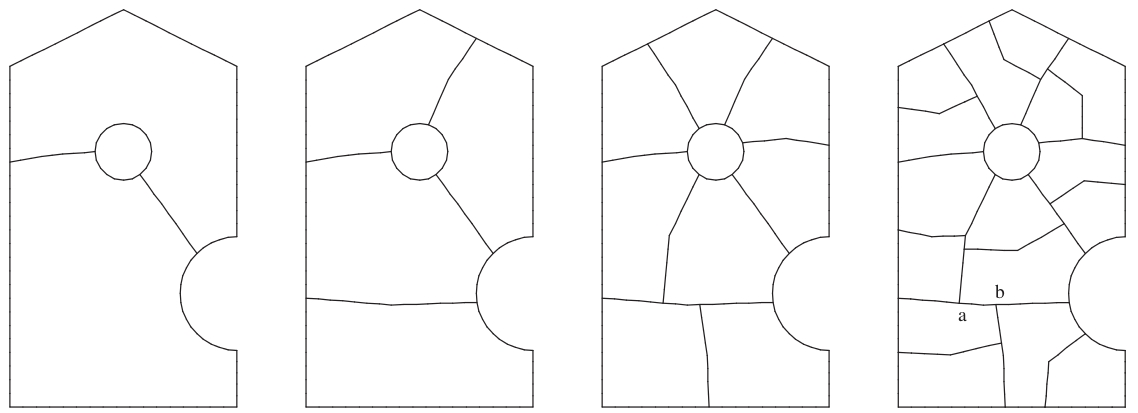
\includegraphics[width=0.9\textwidth]{imagem4}
     \caption{Partições em 2, 4, 8 e 16. \cite{bib:Leonidas06}.}
     \label{fig:imagem4}
 \end{figure}

Através do grafo formado, os planos de corte são posicionados e os subdomínios formados. A Figura~\ref{fig:imagem4} mostra o resultado de decomposições para quantidades diferentes de subdomínios. Após isso a geração da malha interna poderá ser realizada.

\section{Decomposição baseada em \textit{bounding Box}}

Em \cite{bib:Glut08}, é apresentada uma técnica para malhas tridimensionais. Essa é uma abordagem baseada na decomposição geométrica onde a entrada é uma malha de superfície. Aqui são apresentadas duas técnicas baseadas na \textit{bounding box} gerada a partir da entrada.

A seleção do separador do domínio deve garantir um custo de corte baixo, ou seja, encontrar e posicionar o plano de corte não pode ter um custo computacional alto. Além disso, deve garantir um bom balanceamento de carga e minimizar os elementos conectados por múltiplos subdomínios.

A primeira técnica é baseada na malha de superfície. Para o plano de corte ser criado, é preciso a localização do contorno da malha de superfície e do separador. O contorno é então projetado no separador usando uma função 2D de controle espacial baseada no tamanho das arestas (Figura~\ref{fig:imagem5}).

 \begin{figure}[htbp]
     \centering
     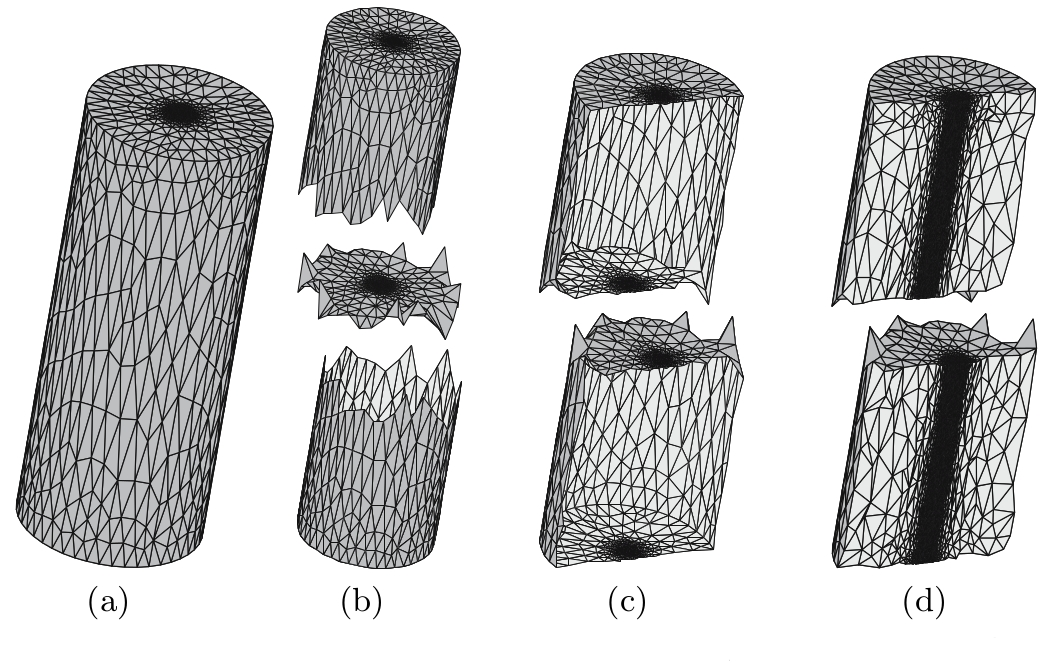
\includegraphics[width=0.9\textwidth]{imagem5}
     \caption{Passos da técnica baseada na malha de superfície. (a) malha de superfície; (b) corte; (c) seção transversal; (d) malha final. \cite{bib:Glut08}.}
     \label{fig:imagem5}
 \end{figure}

A segunda técnica se baseia numa malha volumétrica grosseira. Primeiramente, é feita a geração de uma malha 3D grosseira utilizando alguma função de controle espacial. O posicionamento do plano de corte é feito parecido com a técnica anterior, porém utilizando a malha volumétrica como função espacial (Figura~\ref{fig:imagem6}).

 \begin{figure}[htbp]
     \centering
     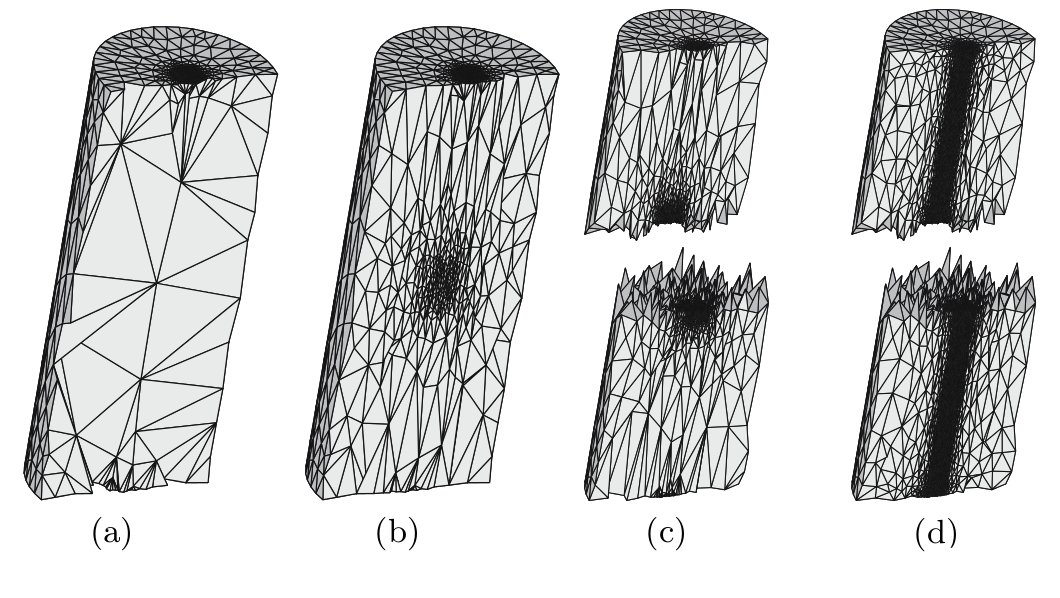
\includegraphics[width=0.9\textwidth]{imagem6}
     \caption{Passos da técnica baseada na malha volumétrica grosseira. (a) malha volumétrica grosseira; (b) refinamento da seção transversal; (c) seção transversal; (d) malha final. \cite{bib:Glut08}.}
     \label{fig:imagem6}
 \end{figure}

Essa técnica depende muito da geometria da entrada já que são utilizadas informações da \textit{bounding box} da entrada. Isso afeta diretamente a criação dos planos de corte e por consequência a malha gerada ao final.

